% \usepackage{graphicx}
% \usepackage{float}
% \usepackage{booktabs} % For professional looking tables

\chapter{State of the Art}

\section*{Introduction}
The rapid advancement of artificial intelligence, particularly in the development of Generative AI (GenAI) and Large Language Models (LLMs), has significantly impacted the field of intelligent systems. These technologies enable the generation of highly personalized and contextually relevant content, marking a pivotal shift in how AI can be applied across various domains. 

A key innovation in this space is the Retrieval-Augmented Generation (RAG) architecture, which synergizes the generative capabilities of LLMs with advanced retrieval mechanisms to enhance the accuracy, relevance, and factual grounding of AI outputs. Central to the effectiveness of RAG are vector stores—specialized databases designed to store and retrieve high-dimensional vector embeddings, thereby enabling efficient semantic search and retrieval processes. 

This chapter provides an in-depth exploration of these core technologies. It begins with the evolution and capabilities of LLMs, followed by the principles and applications of RAG architectures. Furthermore, it examines the critical role of vector stores in facilitating efficient information retrieval, establishing the theoretical foundation for the architectural decisions and innovations introduced in this project.

\section{Large Language Models}

\subsection{Overview}
Language is the fundamental medium for human communication and interaction with machines. The evolution of language models—from early statistical methods to neural approaches, and ultimately to modern LLMs—has revolutionized Natural Language Processing (NLP). The advent of transformer architectures, coupled with enhanced computational capabilities and the availability of vast training corpora, has enabled LLMs to exhibit human-level performance across a myriad of language tasks \cite{ref1, ref2}. 

LLMs are uniquely capable of processing and generating coherent text, demonstrating remarkable generalization across multiple tasks, including translation, summarization, and open-domain question answering. These models have grown exponentially in both complexity and capability, transitioning from standard Pre-trained Language Models (PLMs) to massive LLMs that often comprise tens to hundreds of billions of parameters, trained on datasets spanning gigabytes to terabytes.

\begin{figure}[H]
    \centering
    \IfFileExists{Figures/llm_evolution.png}{
        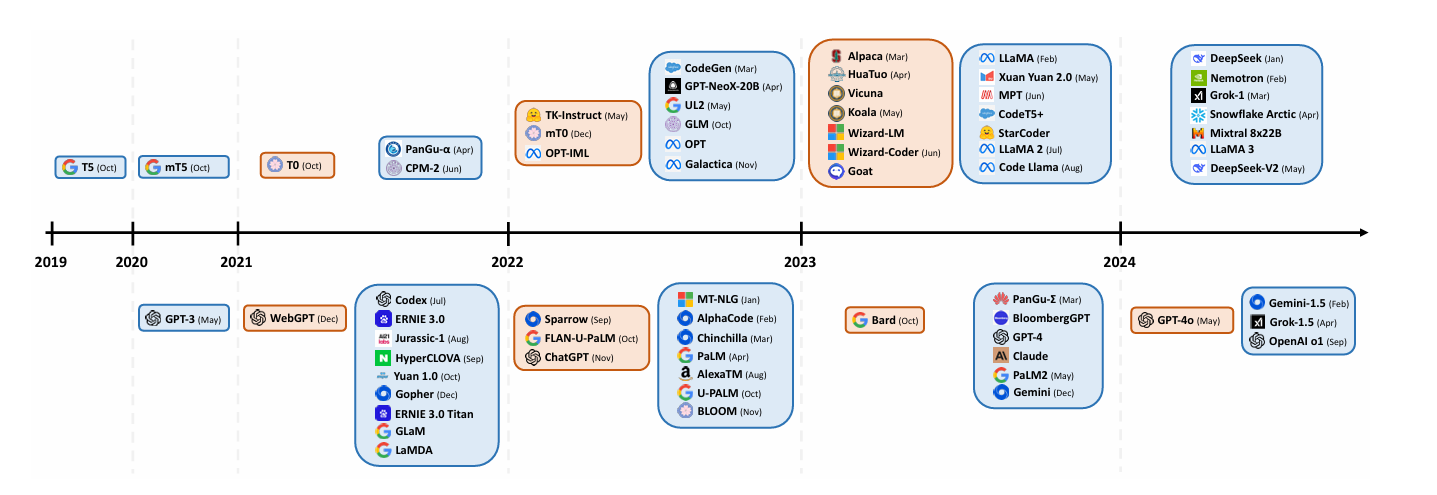
\includegraphics[width=0.85\textwidth, keepaspectratio]{Figures/llm_evolution.png}
    }{
        \framebox[0.85\textwidth]{\rule{0pt}{150pt} \textbf{Missing Image:} llm\_evolution.png}
    }
    \caption{The evolution of Large Language Models.}
    \label{fig:llm_evolution}
\end{figure}

\subsection{Advancements and Capabilities}
LLMs have demonstrated emergent abilities—such as zero-shot reasoning, logical decision-making, and in-context learning—which arise from their massive scale rather than explicit task-specific training. These capabilities allow LLMs to perform complex operations with minimal task-specific data, showcasing their profound generalization potential. Fine-tuning and alignment techniques (such as RLHF) further enhance their performance, enabling them to strictly follow user intent and generate highly accurate, safe responses. 

Moreover, LLMs have shown significant improvements in multi-tasking and adapting to novel contexts. This versatility has positioned them as indispensable tools across diverse industries, ranging from healthcare to finance and legal technology. These advancements underscore the growing importance of LLMs as the cognitive engines of modern AI-driven applications.

\subsection{Challenges and Opportunities}
Despite their undeniable success, LLMs face significant operational challenges, including high computational costs, slow inference latency, and substantial hardware requirements. These limitations have spurred intensive research into more efficient architectures, model compression techniques, and parameter-efficient fine-tuning strategies designed to make LLMs more accessible and practical for broader commercial applications. Methods such as model distillation, structured pruning, and weight quantization are actively being explored to reduce the immense resource intensity of these models. 

One of the most critical challenges LLMs face is managing large-scale input data. While state-of-the-art LLMs can possess context windows of up to 2 million tokens, enterprise knowledge bases often span millions of documents, dwarfing these limits. This discrepancy restricts the ability of LLMs to process entire organizational datasets directly in a single inference step, complicating tasks that require simultaneous access to vast, dispersed information. 

Additionally, the processing time for an LLM query is highly sensitive to the length of the input context. Longer queries demand significantly more computation because the self-attention mechanism processes each token, resulting in increased latency and higher financial costs. Consequently, handling extremely long contexts can become prohibitively expensive, particularly for applications requiring real-time responsiveness or frequent large-scale queries. 

Furthermore, ensuring the ethical deployment of LLMs, mitigating algorithmic biases, and preventing the generation of misleading or harmful outputs remain critical concerns. Overcoming these hurdles presents rich opportunities for ongoing research and engineering innovation.

\begin{table}[H]
    \centering
    \resizebox{\textwidth}{!}{
    \begin{tabular}{l c c c c}
        \toprule
        \textbf{Model} & \textbf{Context Window} & \textbf{Cost (USD/1M Tokens)} & \textbf{Tokens/s} & \textbf{First Chunk (s)} \\
        \midrule
        GPT-4o & 128k & \$7.50 & 97.4 & 0.45 \\
        GPT-4 Turbo & 128k & \$15.00 & 31.9 & 0.60 \\
        GPT-3.5 Turbo & 16k & \$0.75 & 88.6 & 0.38 \\
        Gemini 1.5 Pro & 2M & \$5.25 & 64.6 & 1.05 \\
        Llama 3.1 405B & 128k & \$4.50 & 29.4 & 0.66 \\
        Claude 3.5 Sonnet & 200k & \$6.00 & 76.5 & 1.32 \\
        Mistral Large 2 & 128k & \$4.50 & 36.8 & 0.51 \\
        Mixtral 8x22B & 65k & \$1.20 & 63.3 & 0.34 \\
        \bottomrule
    \end{tabular}
    }
    \caption{Comparison of Selected Models Based on Context Window, Cost, and Performance.}
    \label{tab:model_comparison}
\end{table}

\subsection{Conclusion}
LLMs represent a monumental advancement in Natural Language Processing, offering unprecedented capabilities in text comprehension and generation. However, the operational challenges associated with their deployment—including computational efficiency, context window limitations, query processing latency, and ethical considerations—highlight the pressing need for continued innovation in model architecture and augmentation methodologies.

\section{Vector Stores}

\subsection{Introduction}
While LLMs have made significant strides, their inherent limitations in handling vast amounts of raw input data and long-tail queries remain a crucial bottleneck. Fortunately, emerging architectural paradigms are addressing this issue by providing highly sophisticated mechanisms for managing and accessing large-scale information dynamically during inference. These advancements promise to unlock the full potential of LLMs, enabling them to bypass strict token limits. In the following sections, we will explore vector storage—a groundbreaking architecture that fundamentally redefines large-scale data retrieval for generative AI models.

\subsection{Embeddings and Their Importance}
A vector store is a specialized database engineered to store and efficiently query dense vector embeddings, which are high-dimensional mathematical representations of unstructured data. These embeddings accurately capture the semantic meaning of complex information—such as text, images, or audio—and are paramount for applications requiring rapid, context-aware information retrieval based on semantic similarity rather than mere keyword matching.

Embeddings distill the semantic and syntactic content of data into a continuous vector space that machine learning models can process optimally. They empower systems to execute semantic searches by calculating the mathematical distance (e.g., cosine similarity) between vectors in high-dimensional space. Typically generated by deep neural networks such as BERT or BGE, these vectors encode the intricate relationships between distinct concepts. 

Within this vector space, semantically similar concepts are positioned in close geometric proximity. For instance, synonyms like "contract" and "agreement" would yield embeddings located near one another, reflecting their shared contextual meaning. This capability is absolutely essential for applications demanding high-precision, contextually relevant information retrieval.

\begin{figure}[H]
    \centering
    \IfFileExists{Figures/embedding_space.png}{
        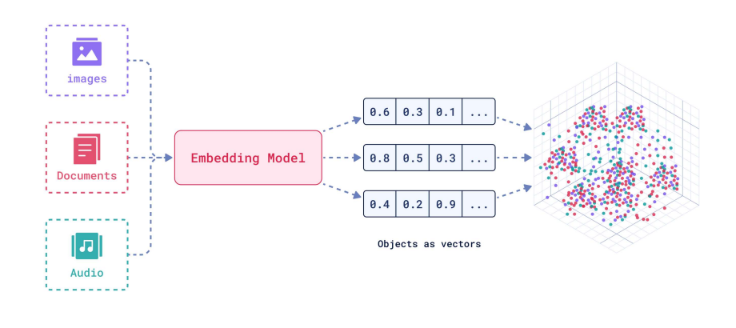
\includegraphics[width=0.7\textwidth, keepaspectratio]{Figures/embedding_space.png}
    }{
        \framebox[0.7\textwidth]{\rule{0pt}{150pt} \textbf{Missing Image:} embedding\_space.png}
    }
    \caption{Illustration of embedding vectors in a high-dimensional semantic space.}
    \label{fig:embedding_space}
\end{figure}

\subsection{Memory and Efficiency Considerations}
The high-dimensional nature of vector embeddings—often consisting of hundreds or thousands of floating-point dimensions—can impose severe memory constraints on the hosting infrastructure. For example, a single 1024-dimensional vector stored as 32-bit floating-point numbers requires approximately 4 KB of memory. As an enterprise database scales into millions of vectors, the active memory demands become substantial. 

To mitigate these memory overheads and accelerate retrieval speeds, sophisticated techniques such as Product Quantization or Binary Quantization are frequently employed. These approaches compress the vectors, drastically reducing their memory footprint while preserving sufficient topological information to guarantee effective retrieval. Converting a 1536-dimensional vector to a binary format, for instance, can reduce its memory requirement by a factor of 40, concurrently accelerating the dot-product calculations required for search. Despite this aggressive compression, high recall accuracy can be maintained by implementing a two-stage pipeline: utilizing compressed vectors for the initial rapid search, and full-precision vectors (or Cross-Encoders) for final ranking.

\subsection{HNSW Algorithm in Vector Stores}
The Hierarchical Navigable Small World (HNSW) algorithm is a state-of-the-art methodology for Approximate Nearest Neighbor (ANN) search, significantly augmenting the query performance of modern vector stores. Traditional brute-force search approaches possess a time complexity of $\mathcal{O}(N)$, rendering them highly impractical for massive datasets. HNSW successfully reduces this search complexity to $\mathcal{O}(\log N)$, enabling sub-millisecond retrieval times. 

The HNSW algorithm organizes vector data into multiple hierarchical layers, each representing a varying level of abstraction and connectivity. The foundational bottom layer contains all data points and is densely interconnected, whereas the upper layers contain exponentially fewer points and longer connections, forming a navigational hierarchy. During a search, the algorithm traverses the sparse upper layers to rapidly locate the general vicinity of the target. Once this approximate region is identified, the search cascades into the denser lower layers to pinpoint the exact nearest neighbors.

The spatial memory complexity of HNSW remains $\mathcal{O}(N)$, as each embedded point maintains a fixed maximum number of connections, ensuring memory consumption grows linearly rather than exponentially. This architectural elegance makes HNSW the industry standard for large-scale, high-velocity semantic retrieval.

\begin{figure}[H]
    \centering
    \IfFileExists{Figures/hnsw_layers.png}{
        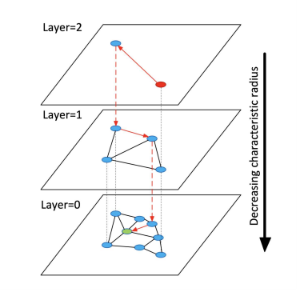
\includegraphics[width=0.75\textwidth, keepaspectratio]{Figures/hnsw_layers.png}
    }{
        \framebox[0.75\textwidth]{\rule{0pt}{150pt} \textbf{Missing Image:} hnsw\_layers.png}
    }
    \caption{Hierarchical representation of the HNSW algorithm layers used in modern Vector Databases.}
    \label{fig:hnsw_layers}
\end{figure}

\subsection{Conclusion}
Vector stores, powered by indexing algorithms like HNSW, represent a paradigm shift in data retrieval technology. By leveraging dense high-dimensional embeddings and logarithmic search algorithms, vector databases offer unparalleled performance for tasks requiring deep semantic understanding. While they demand more active memory than traditional relational databases, vector stores provide the critical speed and accuracy necessary to support next-generation AI applications, from enterprise semantic search to robust data analysis.

\section{RAG Architecture}

\subsection{Introduction}
Large pre-trained language models excel at internalizing vast quantities of factual knowledge within their parameters, achieving remarkable zero-shot performance across various NLP domains. However, they frequently struggle to access and manipulate this latent knowledge accurately, particularly in knowledge-intensive or highly specialized tasks (such as legal reasoning). This architectural limitation becomes glaringly evident when models hallucinate facts, fail to provide up-to-date information, lack the ability to cite provenance for their outputs, or require constant, expensive retraining to update their internal knowledge base. 

Retrieval-Augmented Generation (RAG) elegantly resolves these fundamental challenges by integrating pre-trained parametric memory (the LLM) with dynamic, non-parametric memory (a vector database). In a RAG architecture, a generative model is actively fed by a neural retriever that searches a dense vector index representing a massive external corpus (e.g., millions of legal documents). This architecture empowers the system to dynamically fetch the most relevant, up-to-date information strictly during the inference generation process, resulting in highly specific, diverse, and empirically factual outputs. 

By injecting a deterministic retrieval mechanism directly into the prompt pipeline, RAG models consistently demonstrate state-of-the-art performance in complex NLP tasks, dramatically outperforming parametric-only models while completely resolving the issues of knowledge provenance and hallucination.

\begin{figure}[H]
    \centering
    \IfFileExists{Figures/rag_architecture.jpg}{
        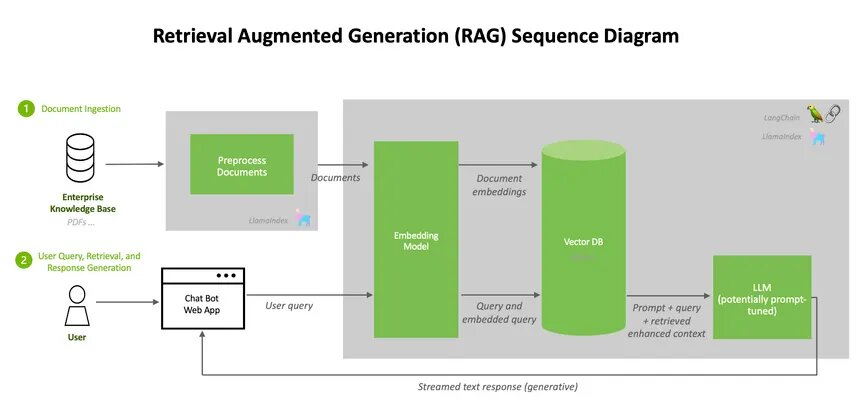
\includegraphics[width=0.85\textwidth, keepaspectratio]{Figures/rag_architecture.jpg}
    }{
        \framebox[0.85\textwidth]{\rule{0pt}{150pt} \textbf{Missing Image:} rag\_architecture.jpg}
    }
    \caption{The standard Retrieval-Augmented Generation (RAG) architecture combining an LLM with an external vector retrieval mechanism.}
    \label{fig:rag_architecture}
\end{figure}

\subsection{The Necessity of RAG Architecture}
Traditional language models rely exclusively on the static information encoded within their neural weights during the pre-training phase. While these models perform admirably on general conversational tasks, they fail critically on tasks demanding domain-specific, proprietary, or temporally recent information. An un-augmented model will frequently generate outdated or entirely fabricated responses because the knowledge it acquired during pre-training is inherently frozen in time and inherently generalized. 

RAG architectures mitigate these limitations by decoupling knowledge storage from language generation. By integrating a dedicated retrieval mechanism, the model is permitted to query external, proprietary knowledge bases on-the-fly. This guarantees that the LLM is constantly grounded by accurate, contextually appropriate, and highly pertinent data fetched directly from a verified repository, effectively turning the LLM from a "memorizer" into an advanced "synthesizer" of factual information.

\subsection{Conclusion}
The RAG architecture, fundamentally underpinned by high-performance vector stores, constitutes a major breakthrough in the deployment of Enterprise AI. By fusing the reasoning capabilities of pre-trained language models with the deterministic accuracy of semantic retrieval mechanisms, RAG guarantees the generation of contextually aware and factually grounded outputs. Consequently, RAG serves as the definitive architecture for deploying secure, trustworthy AI applications in critical sectors such as law, medicine, and finance.